\section{Sentinel-1影像预处理实验}

\subsection{数据获取与查看}
本次使用的实验数据为S1A\_IW\_GRDH\_1SDV\_20210326T095454\_20210326T095519\_037\-168\_046065\_D714.safe, S1A可知该数据来自哨兵一号A星, IW表示数据获取模式, GRDH表示高分辨率的GRD数据, 1S表示标准1级处理产品, DH表示极化方式, 双极化HH+HV; 后面两个日期分别表示数据的开始和结束时间; 037168表示绝对轨道号; 046065表示任务数据的标识符; D714为产品唯一识别码. 数据的获取如图\ref{fig:0301}所示:

\begin{figure}[!htbp]
    \centering
    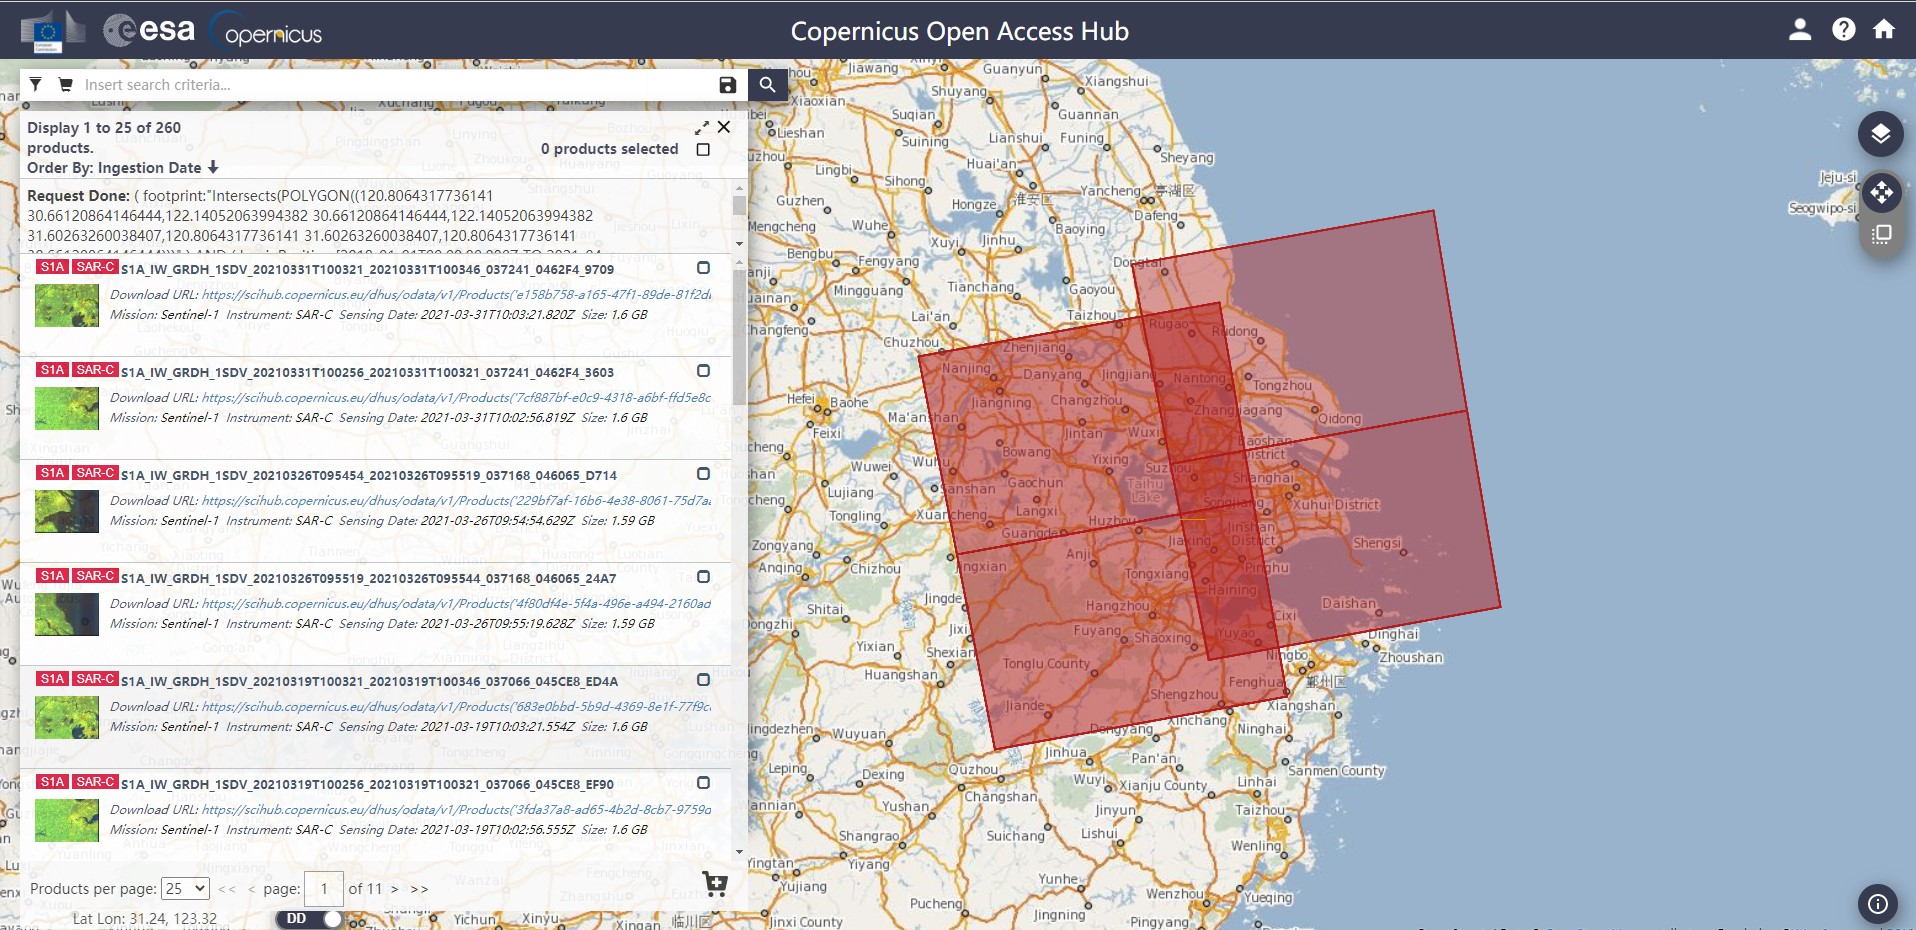
\includegraphics[width=0.8\textwidth]{pic/chap0301.jpg}
    \caption{数据获取}
    \label{fig:0301}
\end{figure}

\begin{figure}[ht]
    \centering
    \subfloat[数据波段]{\label{fig:0302a}
    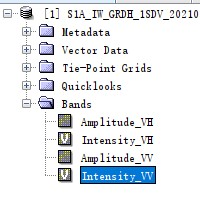
\includegraphics[height=10em]{pic/chap0302a.jpg}}
    \qquad
    \subfloat[VH强度]{\label{fig:0302b}
    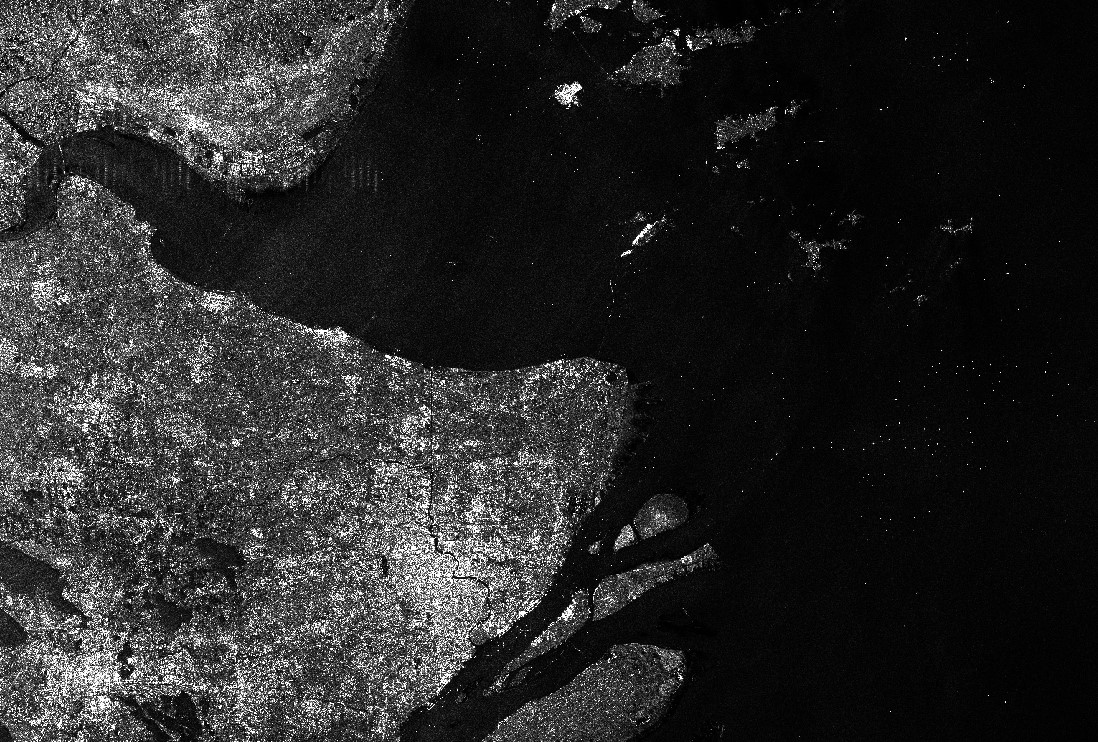
\includegraphics[height=10em]{pic/chap0302b.jpg}} 
    \caption{数据显示}
    \label{fig:0302}
\end{figure}

在欧空局SNAP软件中打开, 如图\ref{fig:0302}, 在\subref{fig:0302a}中可见4个波段, 分别为极化方式为VV, VH的振幅与之对应的强度波段, 注意Intensity\_VH前面有``V''的标志(V是``Virtual''的前缀, 虚拟之意), 这表示该波段是在内存中临时产生虚拟的波段, 不是实际存储在硬盘的波段; 在图\subref{fig:0302b}中可见VH强度显示效果.

\subsection{轨道校正}
该操作会自动下载精确的轨道文件并更新Sentinel-1卫星数据中元数据文件(.xml)中的Sent\-inel-1卫星轨道状态信息, 默认的元数据文件中轨道状态数据精度不是很高. 这个精确的轨道文件通常需要两周左右才能产生, 一般来说, 如果可以更新更精确的轨道位置, 这个操作应该做, 特别是在需要较高的配准处理时. 注意要保持联网, 才能获取精确轨道文件, 其操作如图\ref{fig:0303}所示:

\begin{figure}[ht]
    \centering
    \subfloat[]{\label{fig:0303a}
    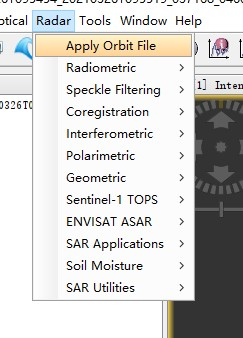
\includegraphics[height=15em]{pic/chap0303a.jpg}}
    \qquad
    \subfloat[]{\label{fig:0303b}
    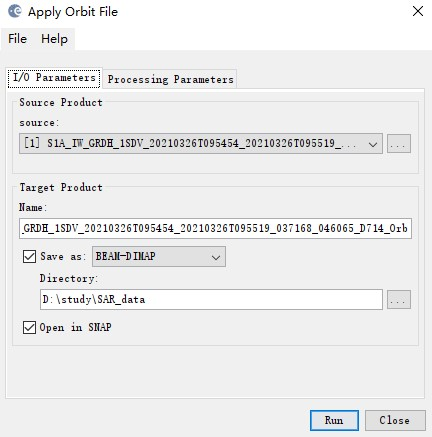
\includegraphics[height=15em]{pic/chap0303b.jpg}}
    \caption{轨道校正}
    \label{fig:0303}
\end{figure}

设置好参数, 点击Run即可. 该操作很快, 仅仅替换元数据文件(.xml)的某些内容, 并不会改变其波段内容, 因此, 操作后的影像是相同的.

\subsection{热噪声去除}

热噪声是SAR卫星系统自带的噪声(可以看作背景噪声), SAR是主动成像的, 需要发射机发出电磁波信号(能量), 由于存在波的球面扩散效应, 能量与SAR天线从发出电磁波到接收电磁波所经历的距离平方反比衰减, 而Sentinel-1卫星距地面高度约700km, SAR卫星发射机需要很大功率,因此SAR卫星装置(发射机, 功率放大器, 接收机等)内部的热量(热损耗)不可以忽视的.

针对Sentinel-1的热噪声去除功能已经集成至SNAP软件中. 使用SNAP软件进行处理, 如图\ref{fig:0304a}在命令栏依次选择 ``Radar'' --- ``Radiometric'' --- ``S-1 Themal Noise Removal'', 则可进入热噪声去除功能的选项; 如图\ref{fig:0304b}, 在处理参数中, 切勿勾选 ``Re-Introduce Themal Noise'', 否则会根据天线记录重新生成热噪声. 

\begin{figure}[h]
    \centering
    \subfloat[]{\label{fig:0304a}
    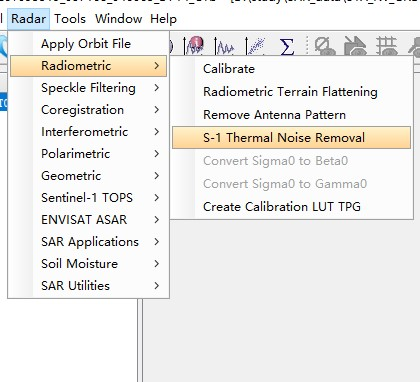
\includegraphics[height=15em]{pic/chap0304a.jpg}}
    \qquad
    \subfloat[]{\label{fig:0304b}
    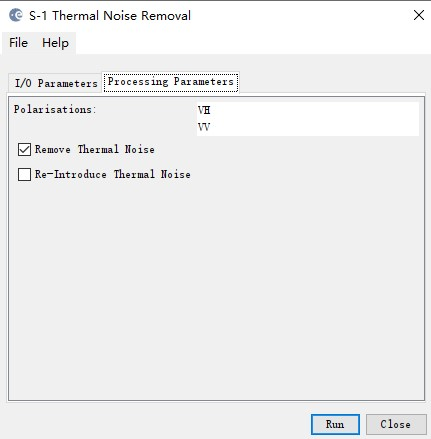
\includegraphics[height=15em]{pic/chap0304b.jpg}}
    \\[12pt]
    \subfloat[]{\label{fig:0304c}
    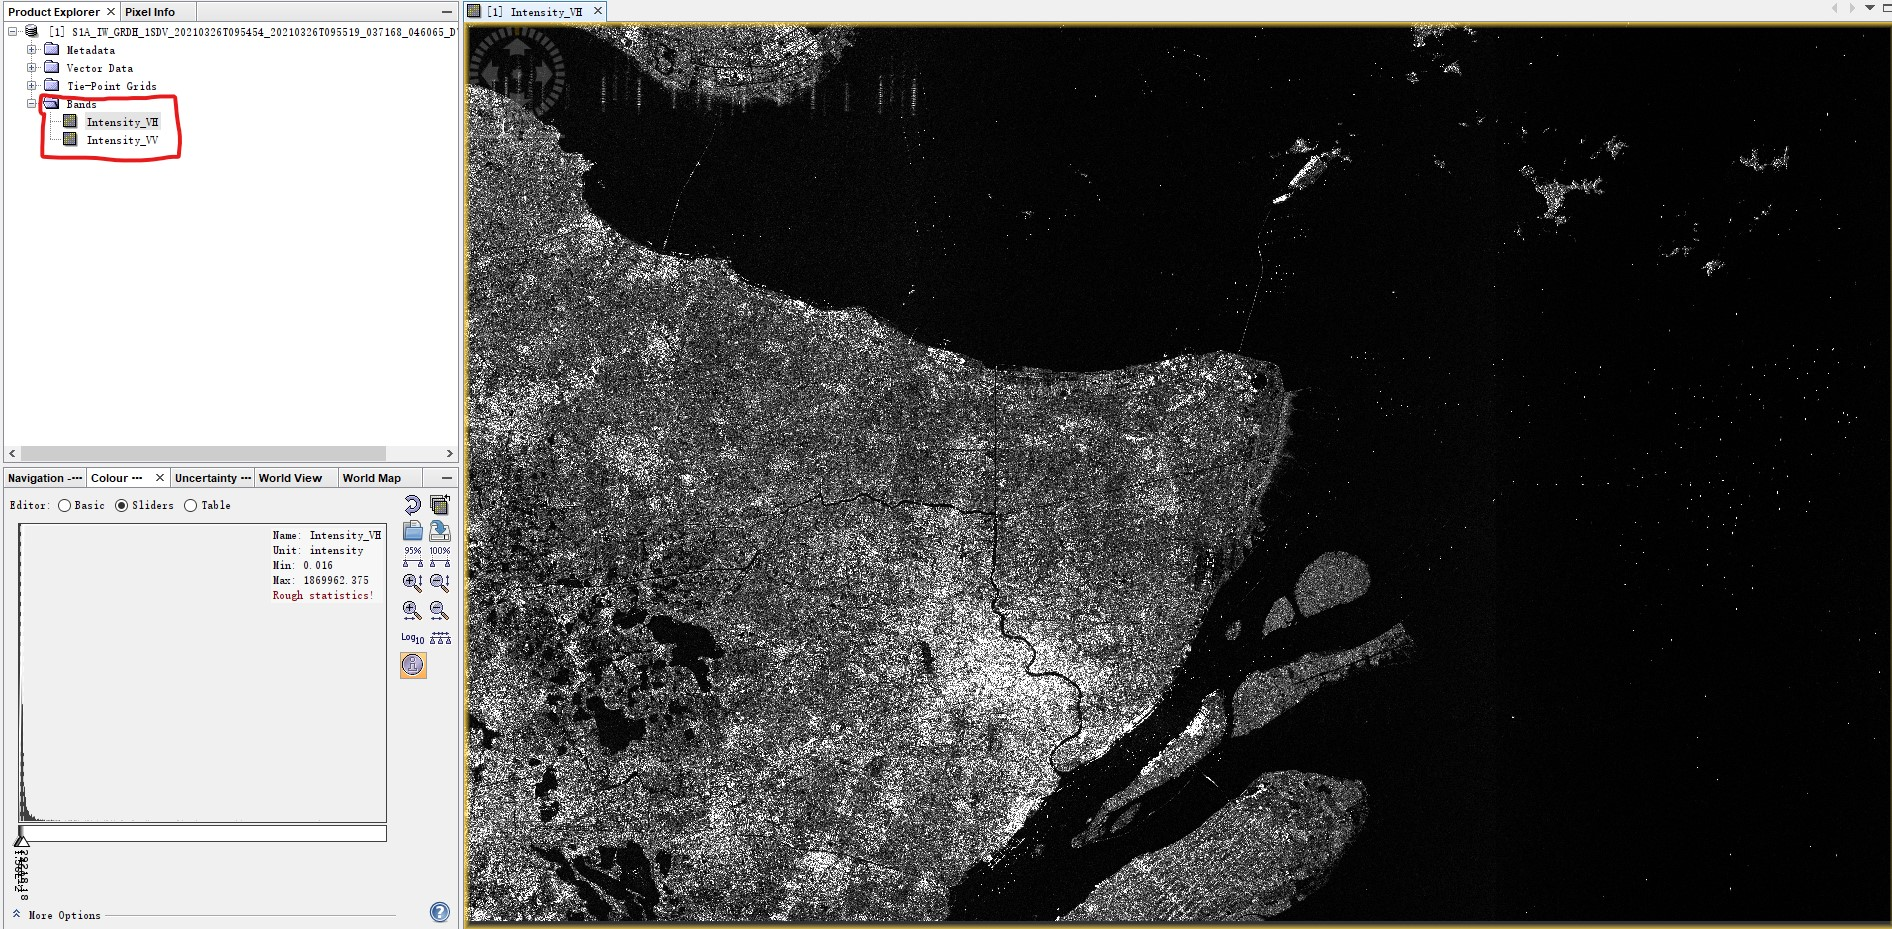
\includegraphics[height=15em]{pic/chap0304c.jpg}}
    \caption{热噪声去除}
    \label{fig:0304}
\end{figure}

如图\ref{fig:0304c}所示, 处理后的影像数据只包含强度信息. 

\subsection{辐射定标}
辐射定标是接收的后向散射信号(能量)转化为有单位的物理量, 比如SAR影像的后向散射系数. 对SAR影像而言, 由于云层的穿透性, 只需要做辐射定标操作即可, 不存在光学影像的大气校正操作. 

如图\ref{fig:0305a}所示在SNAP软件中, 依次选择 ``Radar'' --- ``Radiometric'' --- ``Calibrate''; 如图\ref{fig:0305b}所示, 在处理参数中, 保持默认, 勾选第一项``Output Sigma0 band''. 一般我们都是使用归一化的雷达后向散射系数$\sigma_{0}$即可, $\gamma_{0}$和$\beta_{0}$是在$\sigma_{0}$的基础上改正而得. 定标后结果如图\ref{fig:0305c}所示:

\begin{figure}[ht]
    \centering
    \subfloat[]{\label{fig:0305a}
    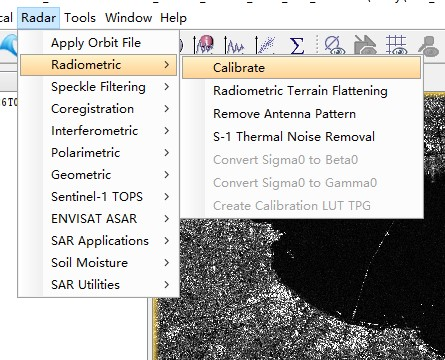
\includegraphics[height=15em]{pic/chap0305a.jpg}}
    \qquad
    \subfloat[]{\label{fig:0305b}
    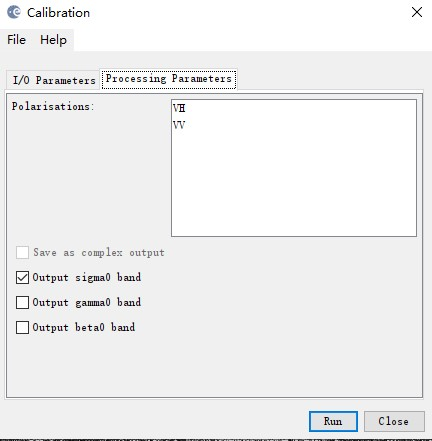
\includegraphics[height=15em]{pic/chap0305b.jpg}}
    \\[12pt]
    \subfloat[]{\label{fig:0305c}
    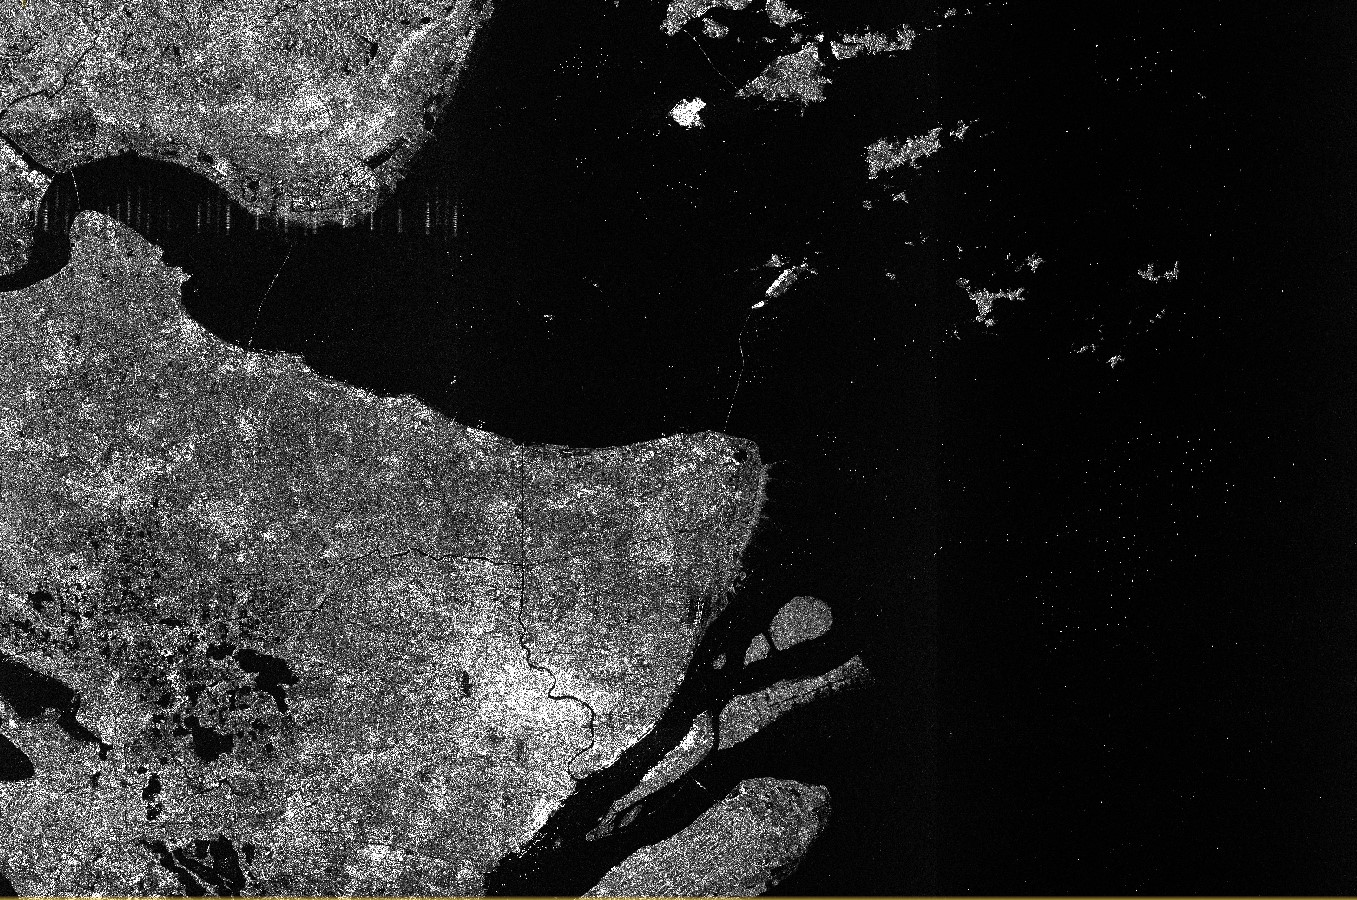
\includegraphics[height=15em]{pic/chap0305c.jpg}}
    \caption{辐射定标}
    \label{fig:0305}
\end{figure}

\newpage
\subsection{相干斑滤波}
相干斑是SAR影像常见的现象. 对于SAR影像分类等应用, 相干斑是噪声, 但对InSAR等来说, 为有效信号. 去除相干斑的滤波器有多种, 本次实验使用目前最常用的相干斑滤波器Refined Lee滤波器, 它是一种自适应滤波器(滤波窗口可以根据区域自动调整), 处理效果较为出色.

\begin{figure}[htbp]
    \centering
    \subfloat[]{\label{fig:0306a}
    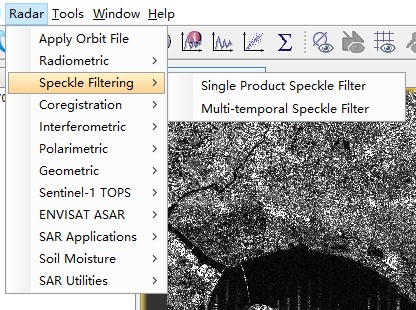
\includegraphics[height=12em]{pic/chap0306a.jpg}}
    \qquad
    \subfloat[]{\label{fig:0306b}
    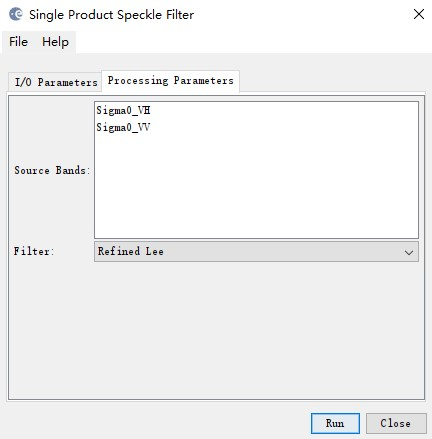
\includegraphics[height=12em]{pic/chap0306b.jpg}}
    \caption{相干斑滤波}
    \label{fig:0306}
\end{figure}

滤波对比结果如图\ref{fig:0307}所示, 图\ref{fig:0307a}为滤波前, 图\ref{fig:0307b}为滤波后; 可明显观察到, 滤除掉相干斑后, 图像斑点变少, 且小邻域内像素值较为均匀.

\begin{figure}[htbp]
    \centering
    \subfloat[滤波前]{\label{fig:0307a}
    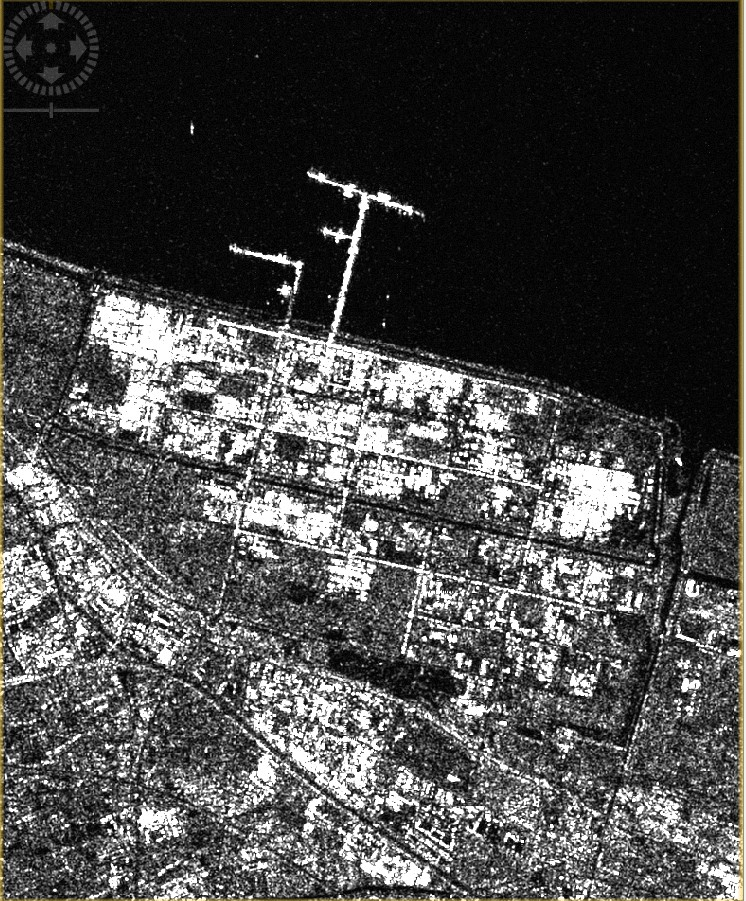
\includegraphics[height=20em]{pic/chap0307a.jpg}}
    \qquad
    \subfloat[滤波后]{\label{fig:0307b}
    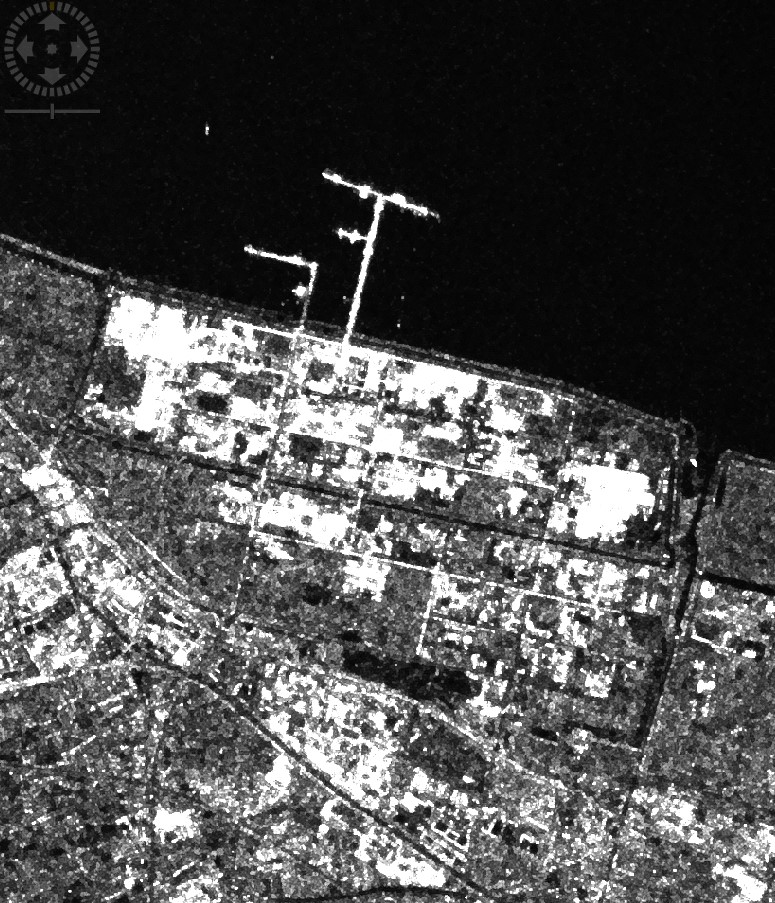
\includegraphics[height=20em]{pic/chap0307b.jpg}}
    \caption{滤波结果}
    \label{fig:0307}
\end{figure}

\subsection{地形校正}

如图\ref{fig:0308a}所示, 在SNAP软件中依次点击, ``Radar'' --- ``Geometric'' --- ``Terrain'' --- ``Correction'' --- ``Range-Doppler Terrain Correction''使用距离多普勒法进行大地校正; 在图\ref{fig:0308b}中设置参数, DEM使用双线性插值, 影像也是用双线性插值重采样, 不能勾选红框部分, 否则没有DEM的数据会被掩膜掉. 该步骤需要联网下载DEM数据. 

\begin{figure}[htbp]
    \centering
    \subfloat[]{\label{fig:0308a}
    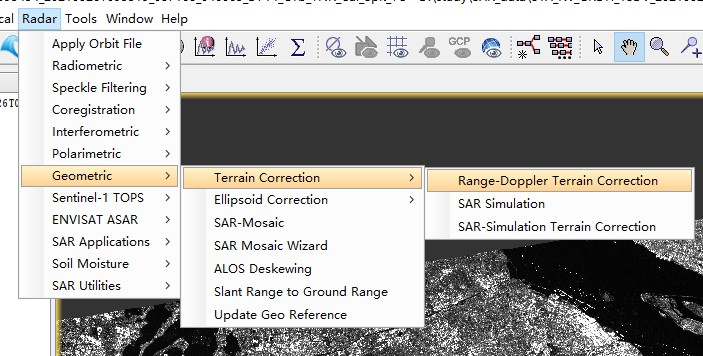
\includegraphics[height=12em]{pic/chap0308a.jpg}}
    \qquad
    \subfloat[]{\label{fig:0308b}
    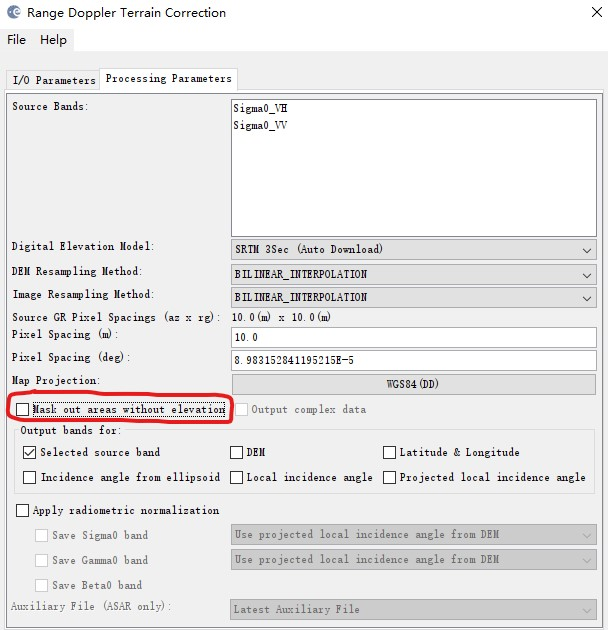
\includegraphics[height=15em]{pic/chap0308b.jpg}}
    \caption{相干斑滤波}
    \label{fig:0308}
\end{figure}

在进行地形校正后, 可明显观察到该影像为上海地区数据, 如图\ref{fig:0309}所示:

\begin{figure}[htbp]
    \centering
    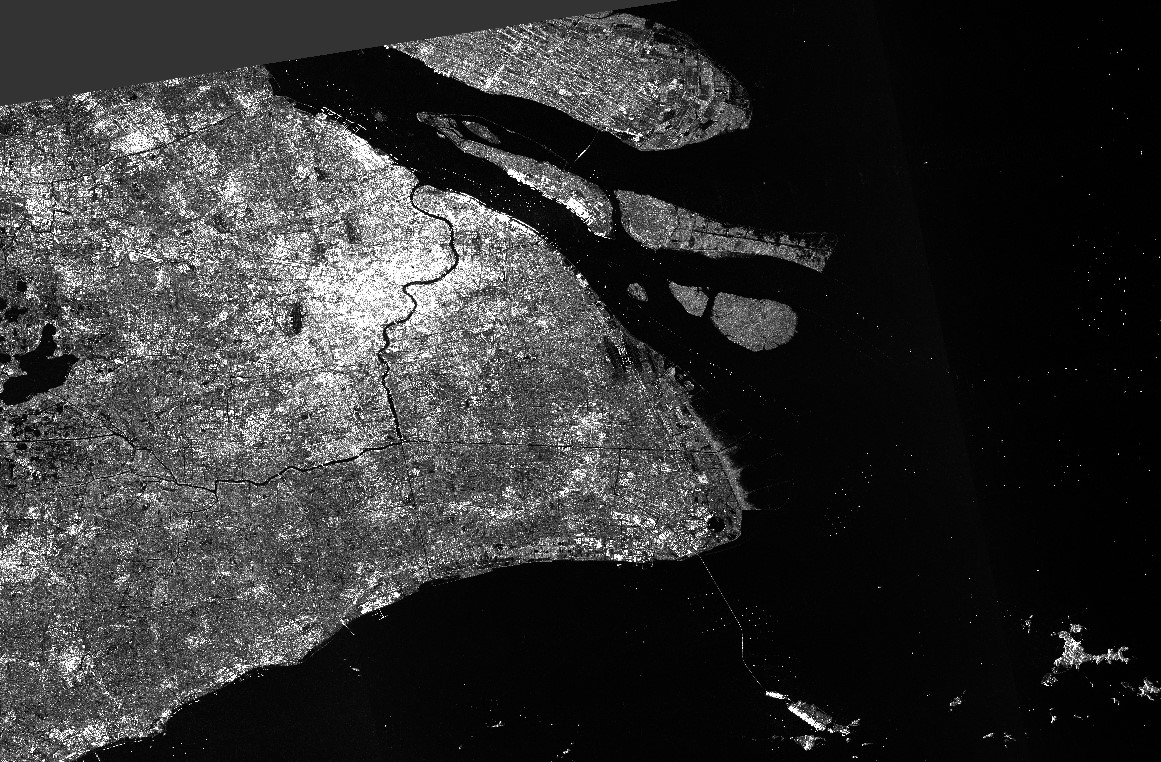
\includegraphics[height=15em]{pic/chap0309.jpg}
    \caption{地形校正结果}
    \label{fig:0309}
\end{figure}

\subsection{分贝化}
上述处理后得到的是线性比例单位的后向散射系数, 但由于传输距离远, 接收器接收的雷达后向散射很小, 其值通常是很小很小的正值. 分贝化公式为:

\begin{equation}
    \sigma_{0}(dB)=10*\lg(\sigma_{0})
\end{equation}

分贝化有几个好处: 一是分贝化的雷达后向散射系数范围近似常见的高斯分布; 二是雷达后向散射系数分贝化后, 数据的存储位数可以变小(可以由双精度的double型数据存为float浮点型数据), 节省存储空间; 三是雷达后向散射系数分贝化后, 可视化以及数据分析上更方便.

具体操作是, ``Raster'' --- ``Data Conversion'' --- ``Converts bands to/from db'', 在经过分贝化操作后, 其结果如图\ref{fig:0310}所示:

\begin{figure}[htbp]
    \centering
    \subfloat[分贝化前]{\label{fig:0310a}
    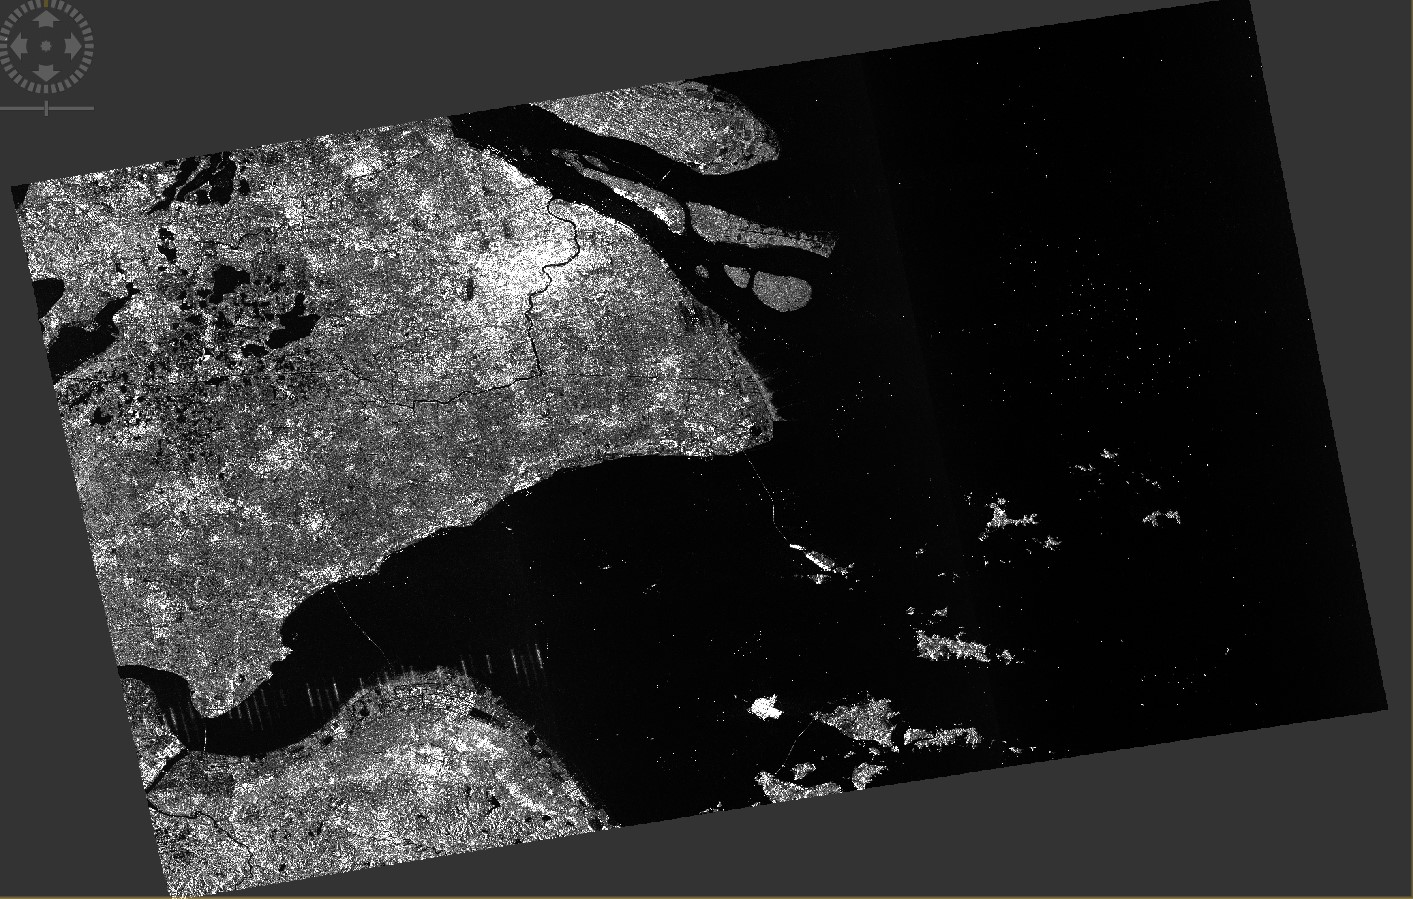
\includegraphics[height=15em]{pic/chap0310a.jpg}}
    \\[12pt]
    \subfloat[分贝化后]{\label{fig:0310b}
    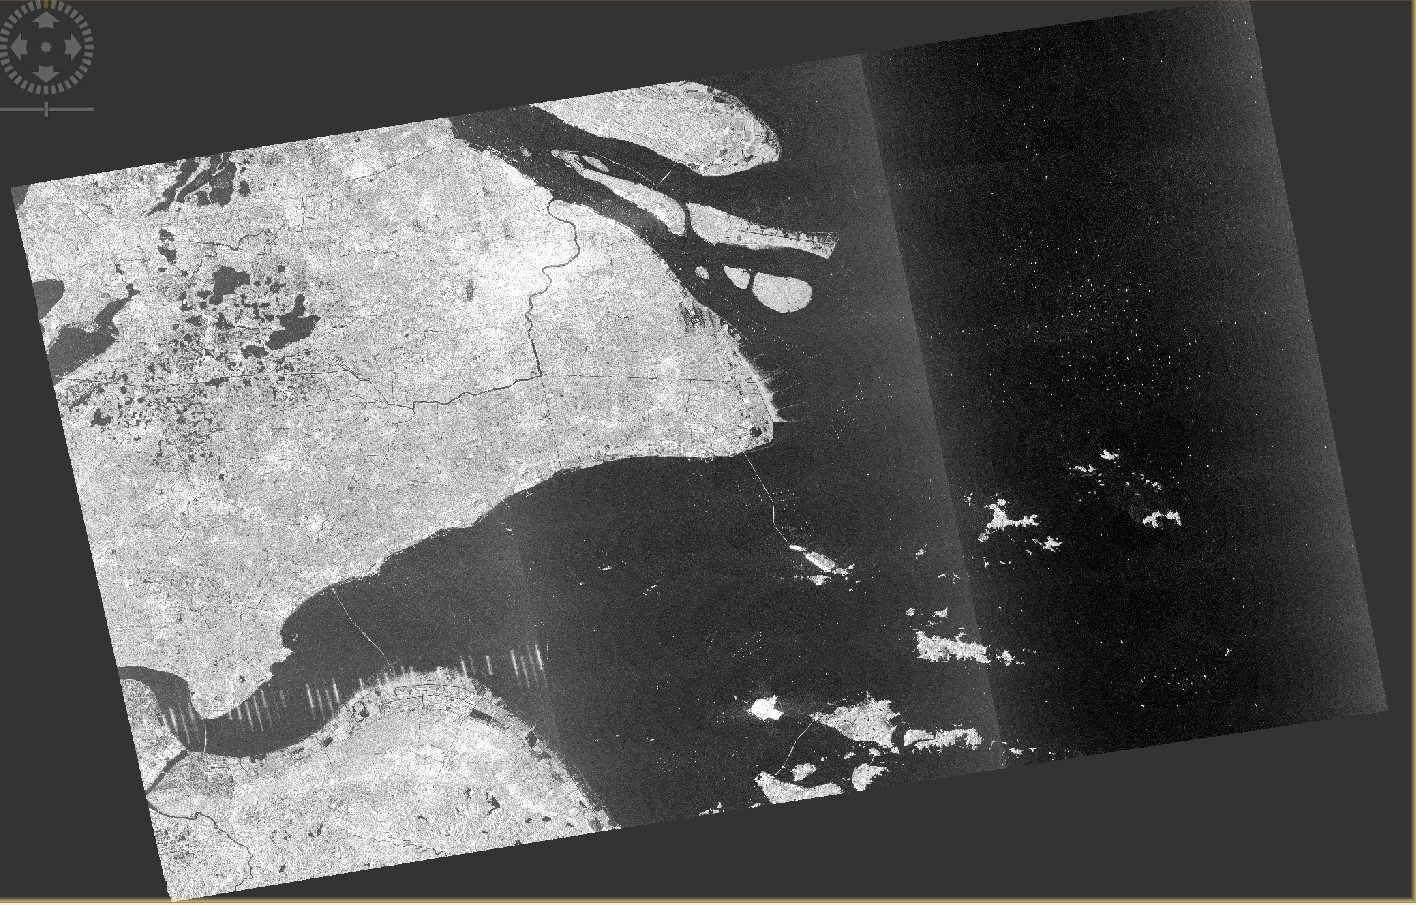
\includegraphics[height=15em]{pic/chap0310b.jpg}}
    \caption{分贝化结果比较}
    \label{fig:0310}
\end{figure}

分贝化前后的图像分布直方图如图\ref{fig:0311}

\begin{figure}[htbp]
    \centering
    \subfloat[分贝化前]{\label{fig:0311a}
    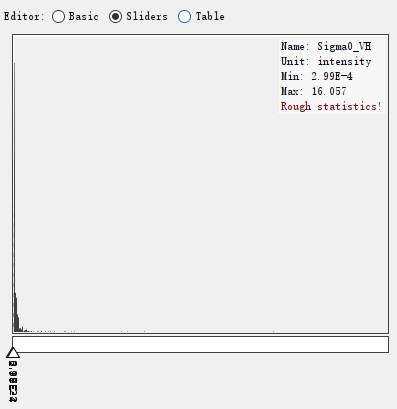
\includegraphics[height=12em]{pic/chap0311a.jpg}}
    \qquad
    \subfloat[分贝化后]{\label{fig:0311b}
    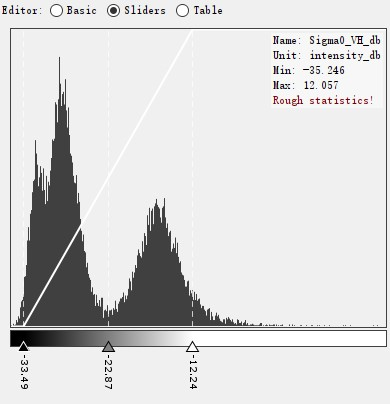
\includegraphics[height=12em]{pic/chap0311b.jpg}}
    \caption{分贝化前后直方图}
    \label{fig:0311}
\end{figure}

观察影像的分布直方图, 分贝化前, 像素值集中在前面, 后向散射系数的值很小; 分贝化后, 像素值呈近似多个高斯分布. 

\newpage
\subsection{影像预处理结果}

至此, Sentinel-1影像预处理完成, 原图为\ref{fig:0312a}, 其最终结果如\ref{fig:0312b}所示.

\begin{figure}[!htbp]
    \centering
    \subfloat[原始影像]{\label{fig:0312a}
    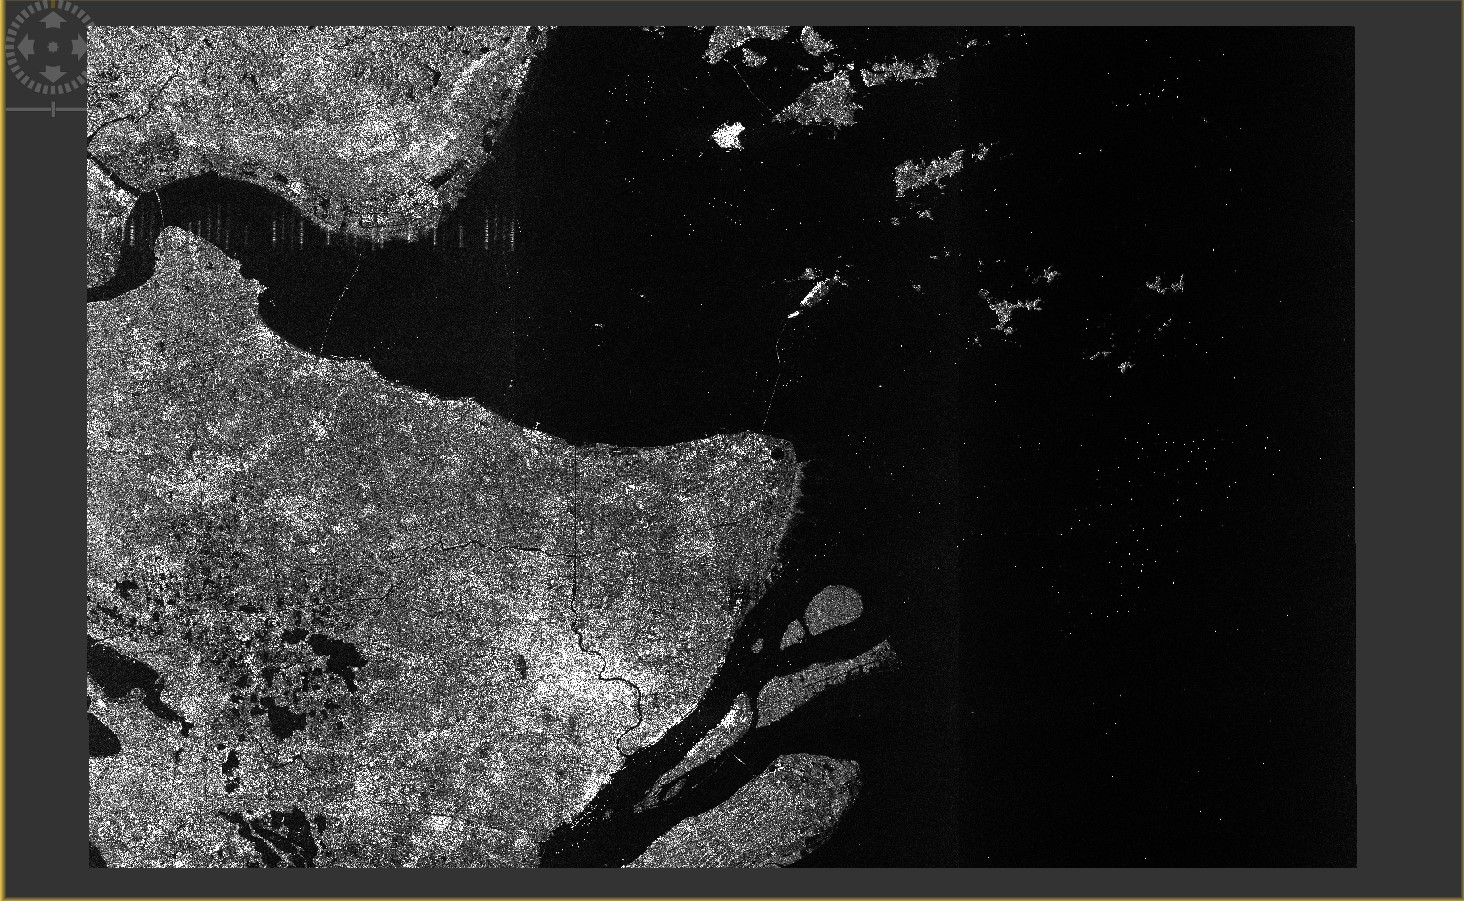
\includegraphics[height=20em]{pic/chap0312a.jpg}}
    \\[12pt]
    \subfloat[预处理后影像]{\label{fig:0312b}
    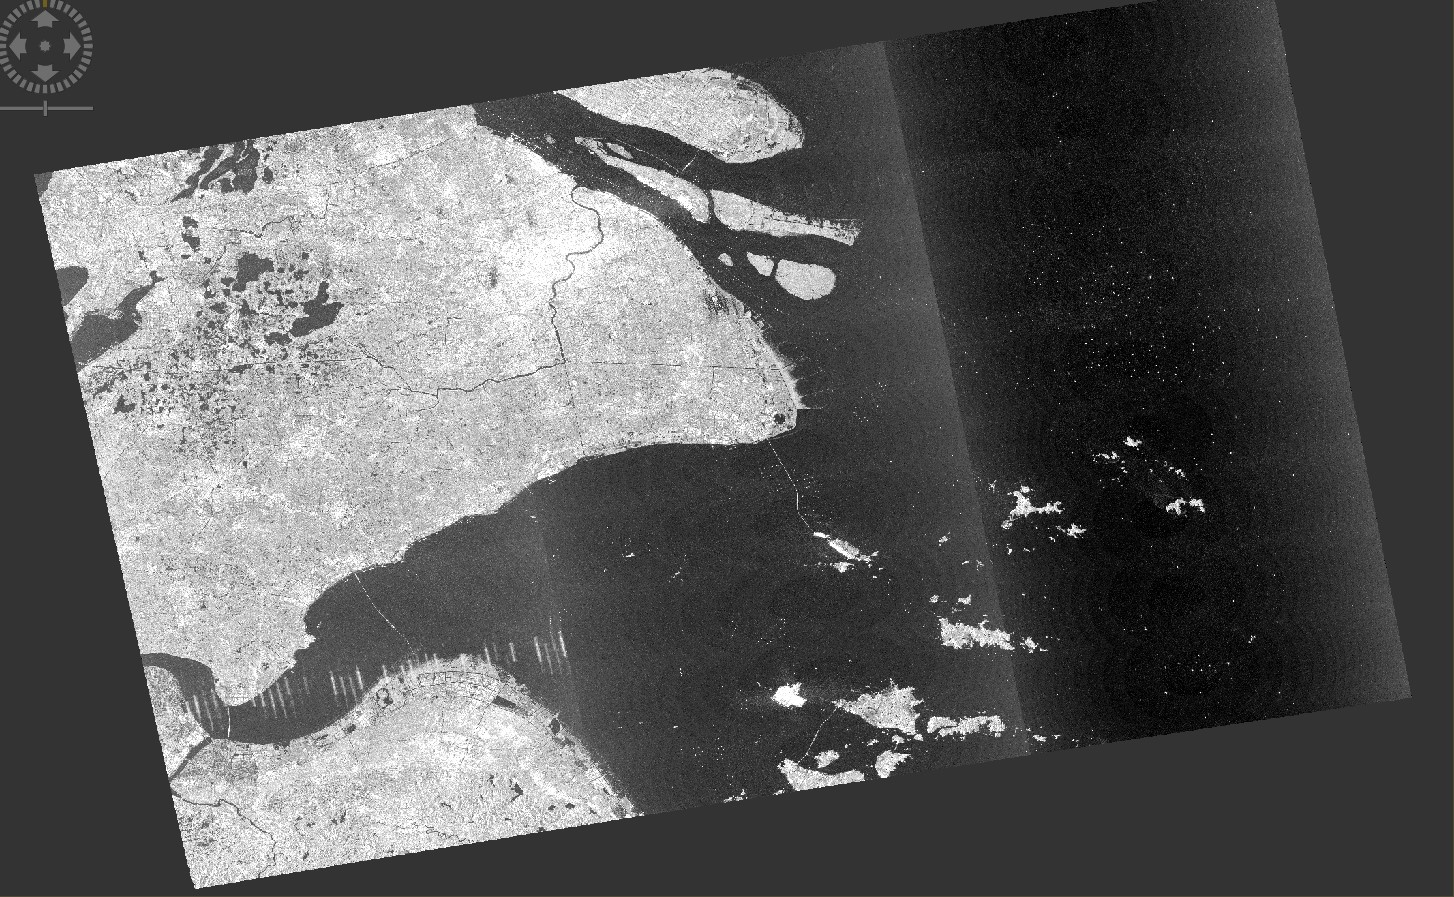
\includegraphics[height=20em]{pic/chap0312b.jpg}}
    \caption{影像预处理结果}
    \label{fig:0312}
\end{figure}